%% =====================================================================
%%  4CroCEE 2027 -- extended abstract template (LaTeX)
%%  Same class as the full paper, with the option "extended":
%%  no Abstract section, keywords directly after the affiliations,
%%  max. 2 pages (500 to 1000 words).  See 4CroCEE_FullPaper.tex for all commands.
%%  Template: Marin Grubišić and Vedran Jagodnik, with the assistance of Claude.
%% =====================================================================
\documentclass[extended]{Definitions/CroCEE}

\title{TITLE (uppercase, max. two lines)}

\author[1]{First Author}
\author[2]{Second Author}
\author{… (first and last name of each author, separated by commas)}

\affiliation[1]{Position, affiliation, e-mail address}
\affiliation[2]{Position, affiliation, e-mail address}

\begin{document}

\maketitle

\keywords{keywords1, keywords2, etc. Authors should suggest about 4--8 keywords for indexing purposes (separated by commas). Keywords are typeset automatically in italics, 10\,pt, by the \texttt{\textbackslash keywords} command.}

This document explains and illustrates how to prepare an extended abstract for the 4\textsuperscript{th} Croatian Conference on Earthquake Engineering -- 4CroCEE 2027 using the LaTeX template. \textbf{Extended abstract can only be submitted for the Engineering Seismology session and the PhD session.}

Extended abstracts should not exceed \textbf{2 pages in length} with 500 to 1000 words. They may include figures, tables, endnotes, acknowledgements, and references. Manuscripts must be written in English. Authors using LaTeX must submit the complete source files \textbf{(.tex, .bib and figure files)} together with the compiled PDF, and should ensure that the formatting complies with the guidelines below before submission. The class option \texttt{extended} in the \texttt{\textbackslash documentclass} command removes the Abstract section and makes the compiler warn if the document exceeds two pages.

\section{General Appearance}

\textbf{The page layout, the 11\,pt Palatino font, the line spacing (exactly 1.2 times the font size), the single-column text and the 1\,cm indentation of the second and the following paragraphs are set by the class file \texttt{crocee.cls}. Do not change the margins, font sizes or spacing, and do not modify the class file.}

Section headings (\texttt{\textbackslash section}, bold 13\,pt; \texttt{\textbackslash subsection}, bold 11\,pt) and the numbering of tables, figures and equations are generated automatically; refer to them with \texttt{\textbackslash tabref}, \texttt{\textbackslash figref} and \texttt{\textbackslash Eqref}. Page numbers are added by the editors.

\subsection{Tables, figures and equations}

Tables are referred to in the text as \tabref{tab:modes} and must be included as part of the text, as shown below. The caption of each table is placed \underline{above} the table, centred, in 10\,pt font; table content is set in 10\,pt font (not smaller than 8\,pt). Tables span the full text width and use the \texttt{booktabs} rules, without vertical lines or shading.

\begin{table}
  \begin{adjustwidth}{-\extralength}{0cm}
  \caption{Dynamic properties of model.}
  \label{tab:modes}
  \begin{tabularx}{\fulllength}{cCCCC}
    \toprule
    \textbf{Mode} & \textbf{T (s)} & \textbf{Mx} & \textbf{My} & \textbf{MRz} \\
    \midrule
    1 & 0.116 & 0     & 0.833 & 0     \\
    2 & 0.087 & 0.755 & 0     & 0.076 \\
    3 & 0.062 & 0.076 & 0     & 0.755 \\
    \bottomrule
  \end{tabularx}
  \end{adjustwidth}
\end{table}

Figures are referred to in the text as \figref{fig:model}. Colour figures can be used, with a minimum resolution of 300 dpi. The caption is placed \underline{below} the figure.

\begin{figure}
  \centering
  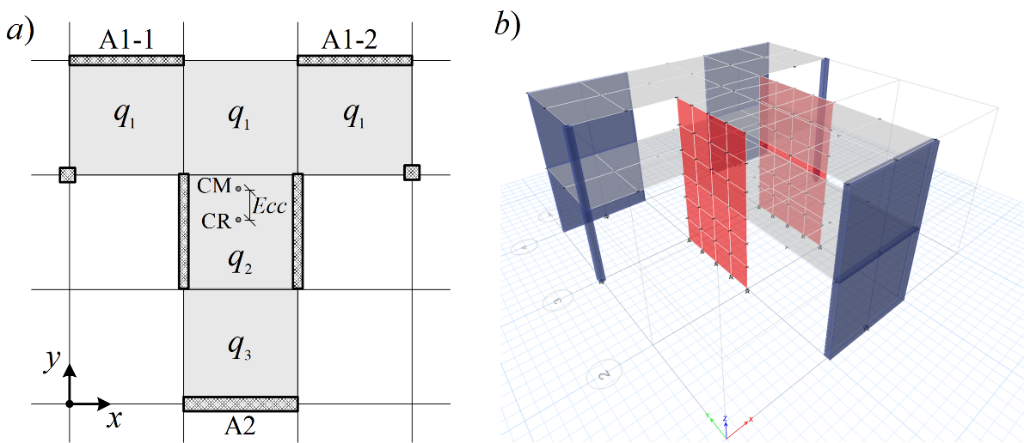
\includegraphics[width=12cm]{Figures/example_figure.png}
  \caption{a) Building plan; b) Numerical model.}
  \label{fig:model}
\end{figure}

Symbols denoting vectors and matrices are set in bold with \texttt{\textbackslash vect} and \texttt{\textbackslash matr}; scalar variables are italic. Equations are centred, numbered automatically and referred to as \Eqref{eq:pythagoras}:
\begin{equation}
  a^2 + b^2 = c^2
  \label{eq:pythagoras}
\end{equation}

\section*{Acknowledgements}

Acknowledgements provide an opportunity to express appreciation to those who contributed significantly to the preparation of the paper. They may be written in free style and must be brief.

\setbibpreamble{References are cited in the text using square brackets \cite{DAyala2003,Bommer2010}, numbered in the order of appearance, and listed at the end in the \emph{Elsevier (numeric, with titles)} style, generated by BibTeX from \texttt{Bibliography/References.bib}; see \texttt{4CroCEE\_FullPaper.tex} for details.}

\bibliographystyle{Definitions/Elsevier}
\bibliography{Bibliography/References}

\end{document}
